\documentclass[xcolor=dvipsnames]{beamer}


\usetheme{Berkeley}

\setbeamertemplate{footline}[frame number]

\usepackage{inputenc}
\usepackage{amsmath}
\usepackage{graphicx}

\title{HLock: Locking IPs at the High-Level Language}
\subtitle{Rafid M., Roshanak M., Mark T. and Farimah F \\ University of Florida \\ Design Automation Conference(DAC) 2021}

\begin{document}
    
    \begin{frame}

        \maketitle

        Presented by \\ Akshay Gopalakrishnan

    \end{frame}

    \begin{frame}{Authors?}


        
    \end{frame}

    \begin{frame}{Outline}

        \begin{itemize}
            \item Security ! 
            \item Security from what ? 
            \item Remedy ? "Lock" parts of the code. 
            \item Lock at High Level description to avoid attackers from succeeding (resiliency).
            \item Results
        \end{itemize}
        
    \end{frame}

    \section{Background}
    \begin{frame}{Security Need}

        \begin{columns}
            
            \begin{column}{0.5\textwidth}
                
                \begin{figure}
                    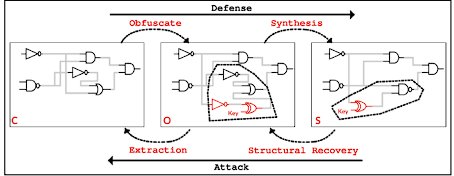
\includegraphics[scale=0.6]{ReverseEng.PNG}
                \end{figure}

            \end{column}

            \begin{column}{0.5\textwidth}
                
                \begin{figure}
                    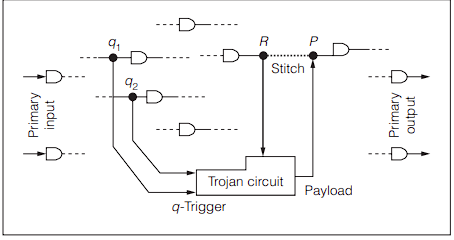
\includegraphics[scale=0.6]{TrojanEx.PNG}
                \end{figure}

            \end{column}

        \end{columns}



        \begin{itemize}
            \item Intellectual Property (IP) blocks of code. 
            \item IP blocks used for Hardware synthesis.
            \item Attacks - eg: Hardware Trojans, Reverse Engineering, etc.
        \end{itemize}
        
    \end{frame}

    \begin{frame}{Security Measures: Locking/Obfuscation}

                
        \begin{figure}
            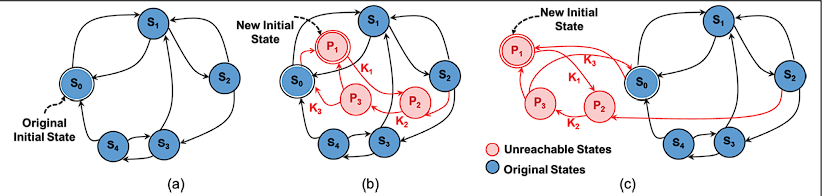
\includegraphics[scale=0.6]{State_Lock.PNG}
        \end{figure}

        
        \begin{itemize}
            \item Modify parts of the hardware specification at the RTL/netlist layer.
            \item The parts work correctly only with another extra input being correct.
            \item This way, "locking" of IP blocks can be achieved.
        \end{itemize}

    \end{frame}

    \begin{frame}{Problem?}

        \begin{itemize}
            \item RTL/netlist layer security not resilient enough.
            \item Obfuscating constant values and branches of RTL are hard to do. 
            \item SAT based/ Machine learning based attacks can easily extract the original design.
        \end{itemize}
        
    \end{frame}

    \section{Main}
    \begin{frame}{Proposed Solution}

        \begin{itemize}
            \item Perform locking/obfuscation at HLS level (C/C++ like) design.
            \item Previous approach exists in these lines, but do not measure resilience to attack and has more overhead.
        \end{itemize}
        
    \end{frame}

    \begin{frame}{Outline}

        \begin{figure}
            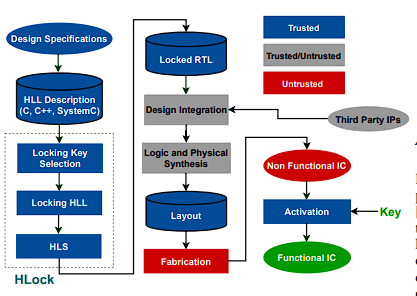
\includegraphics{HLockOverview.PNG}
        \end{figure}
        
    \end{frame}

    \begin{frame}{Locking Different Candidates}

        \begin{figure}
            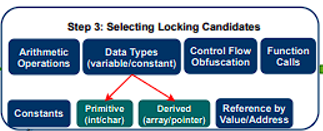
\includegraphics{LockingCandidates.PNG}
        \end{figure}
        
    \end{frame}

    \begin{frame}{Branch Obfuscation}

        \begin{figure}
            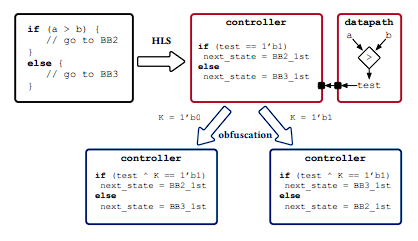
\includegraphics{BranchObfuscation.PNG}
        \end{figure}
        
    \end{frame}

    \begin{frame}{Function Obfuscation}

        Own code sample here.
        
    \end{frame}

    \begin{frame}{Constant Obfuscation}

        \begin{figure}
            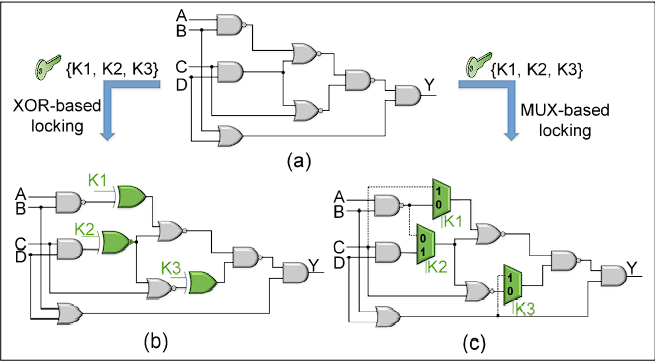
\includegraphics[scale=0.6]{XOR_Lock.PNG}
        \end{figure}
        
    \end{frame}

    \begin{frame}{Whole setup}

        \begin{figure}
            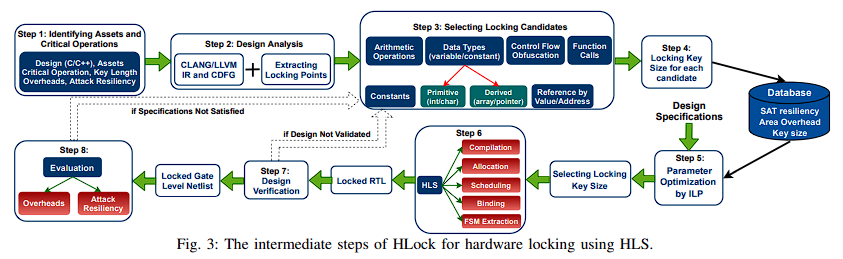
\includegraphics[scale=0.6]{HLockPipeline.PNG}
        \end{figure}
        
    \end{frame}

    \section{Results}
    \begin{frame}{Power consumption and SAT Resiliency}
        \begin{figure}
            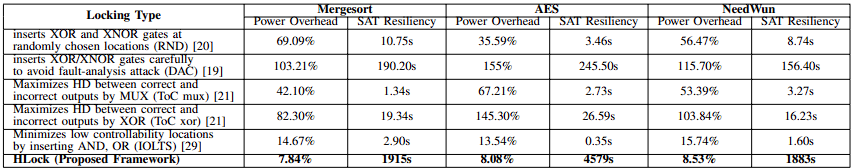
\includegraphics[scale=0.6]{Result_SAT_Power.PNG}
        \end{figure}
    \end{frame}

    \begin{frame}{ML Resiliency}

        \begin{figure}
            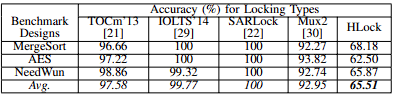
\includegraphics{Result_ML.PNG}
        \end{figure}
        
    \end{frame}

    \section{Conclusion}
    \begin{frame}{Pros and Cons}
        
    \end{frame}

    \begin{frame}{Thank you}

        Useful links:
        
    \end{frame}

\end{document}
